\documentclass[11pt]{article}
\pdfoutput=1
\usepackage[T2A]{fontenc}
\usepackage[utf8]{inputenc}
\usepackage[english, russian]{babel}
\usepackage{NotesTeX_rus}
\usepackage{a4wide}
% Математика
\usepackage{amsmath,amsfonts,amssymb,amsthm,mathtools} 
\usepackage{wasysym}
\usepackage{indentfirst}
\usepackage{a4wide} 
\usepackage[T2A]{fontenc}			% кодировка
\definecolor{block-gray}{gray}{0.90} % уровень прозрачности (1 - максимум)
\newtcolorbox{myquote}{colback=red!5!white,grow to right by=0mm,grow to left by=0mm, boxrule=0pt,boxsep=0pt,breakable} % 1настройки области с изменённым фоном
%Заголовок
%\usepackage{graphix}
%зададим полезные команды:
%скалярное произведение
\newcommand{\scalar}[2]{\left \langle #1,#2\right \rangle}
%выпуклая оболочка
\newcommand{\diag}{\textrm{diag}}
\newcommand{\comp}{\textrm{comp}}
\newcommand{\conv }[0]{\textrm{conv}}
\newcommand{\sgn}[1]{\textrm{sgn}\left(#1\right)}
\newcommand{\Si}[1]{\textrm{Si}\left(#1\right)}

\begin{document}
\thispagestyle{empty}

\begin{center}
\ \vspace{-3cm}

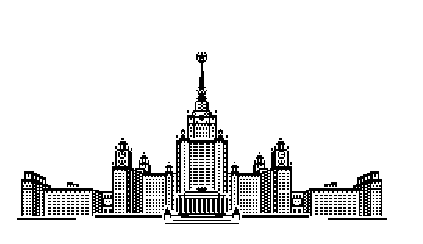
\includegraphics[width=0.5\textwidth]{msu.eps}\\
{\scshape Московский государственный университет имени М.~В.~Ломоносова}\\
Факультет вычислительной математики и кибернетики\\
Кафедра системного анализа

\vfill

{\LARGE Курсовая работа}

\vspace{1cm}

{\LARGE\bfseries <<Динамические системы и модели биологии>>} \\
\vspace{1cm}
{\Large\bfseries <<Часть 1: Динамические системы с дискретным временем>>}
\end{center}

\vspace{1cm}

\begin{flushright}
  \large
  \textit{Студент 315 группы}\\
  И.\,В.~Шамков

  \vspace{5mm}

  \textit{Преподаватель}\\
  к.ф.-м.н., доцент И.\,В.~Востриков
\end{flushright}

\vfill

\begin{center}
Москва, 2022
\end{center}

\newpage
\tableofcontents
\newpage
\section{Постановка задачи}
	\begin{itemize}
	\item {\it Одномерная система:}
	\begin{equation} \label{system_1}
	u_{t+1} =  r \cdot \sqrt{u_t} (1 - a u_t^3), a > 0, r > 0, u_t \in \mathbb{R}_+, \forall t \in \mathbb{Z}_+
	\end{equation}
	\item {\it Двумерная система:}
	\begin{equation} \label{system_2}
	u_{t+1} = r \cdot \sqrt{u_t} (1 - a u_{t+1}^3), a > 0, r > 0, u_t \in \mathbb{R}_+, \forall t \in \mathbb{Z}_+
	\end{equation}
	\end{itemize}
	Необходимые задачи:
\begin{enumerate}
    \item Найти неподвижные точки.
    \item Исследовать устойчивость неподвижных точек в зависимости от значений параметров.
    \item Проверить существование циклов длиной 2 и 3.
    \item В случае существования цикла длиной 3 построить бифуркационную диаграмму.
    \item Построить график показателя Ляпунова в зависимости от значений параметра.
    \item В случае системы с запаздыванием проверить возможность возникновения бифуркации Неймарка-Сакера. 
\end{enumerate}
\newpage
\section{Исследование одношаговой системы}
	\begin{subsection}{Нахождение неподвижных точек}
	Введём определение неподвижной точки для исследования дискретной одношаговой системы \ref{system_1}
	\begin{definition} Точка $u^* \in \mathbb{R} $ называется неподвижной точкой
	системы $ u_{t+1} = f(u_t)$, если $u^* = f(u^*)$, где $f : \mathbb{R} \mapsto \mathbb{R}$.
	\end{definition}
	Рассмотрим $f~= f(u,a,r)~= r\sqrt{u} (1 - a u^3)$. Тогда для нахождения неподвижный точек требуется решить уравнение $f(u,a,r) = u$.
	$$ r\sqrt{u} (1 - a u^3) = u $$
	$$ r\sqrt{u}(1 - a u^3) - u = 0 $$ 
	$$ \sqrt{u} \cdot (r - aru^3 - \sqrt{u}) = 0 $$
	\begin{equation*}	
	\begin{cases}
	u~= 0,
	\\
	(r - aru^3 - \sqrt{u}) = 0
	\\
	\end{cases}
	\end{equation*}
	Из системы следует, что первая неподвижная точка $ u^*_1 = 0$. Исследуем второе уравнение из системы: $r - aru^3 = \sqrt{u} $. Аналитического решения этого уравнения не существует, однако попробуем выяснить количество решений и их зависимость от параметров $a,r$.Рассмотрим функцию $f(u)~= \sqrt{u}$. $g'(u) = \frac{1}{2\sqrt{u}} > 0 $ для $\forall u > 0$ (по условию) $\Rightarrow $ функция $f(u)$ возрастает на $\mathbb{R}_+$. \\
Az	Исследуем функцию $g(u) = r - aru^3 $. Исследуем производную,чтобы найти промежутки возрастания-убывания $g(u)$.$g'(u) = -3aru^2$. Тогда для $\forall a > 0, r > 0$ $g(u)$ убывает на $\mathbb{R}_+$. Следовательно существует единственное некоторое нетривиальное решение $\tilde{u}: f(\tilde{u}) = g(\tilde{u})$.Однако аналитически выразить решение не представляется возможным.
\begin{figure}[H]
\begin{center}
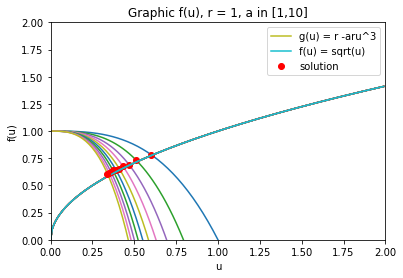
\includegraphics[width=0.5\textwidth]{graphic_2.png}
\caption{Графики $g(u) = r - aru^3$ и $f(u) = \sqrt{u}$ при фиксированном $r=1$ 
\\ и $a \in [1,10]$ красными точками помечено решение уравнения $f(u) = g(u)$} \label{pic_1}
\end{center}
\end{figure}

	\end{subsection}
	\begin{subsection}{Исследование устойчивости неподвижных точек}
	Сначала дадим теоретическую сводку об устойчивости и ассимптотическом устойчивости точек.
	\begin{Commentocre}
	Пусть задана дискретная система: \\
	$u_{t+1} = f(u_t),$ $ f: \mathbb{R}_+ \mapsto \mathbb{R}_+ $.\label{system}\\
	Пусть также задано начальное приближение $u_0$.
	\end{Commentocre}
	\begin{definition}(Устойчивость по Ляпунову) \\
	Неподвижная точка $u^*$ называется \underline{\it устойчивой} точкой по Ляпунову, если: \\
	 для 
	$\forall \varepsilon > 0 \exists \delta=\delta(\varepsilon) > 0 : \forall u_0:
	|u_0 - u^*| < \delta \Rightarrow |u_t - u^*| < \varepsilon $ для $\forall t \in \mathbb{Z}_+ $. Кроме того, если $\lim_{t\to\infty}{f(u_t)} = u^*$, то точка $u^*$ называется \underline{\it ассимптотически устойчивой}.	
	\end{definition}
	\begin{definition}
	Устойчивые неподвижные точки называются \underline{\it аттракторами}, а \\ неустойчивые неподвижные точки называются \underline{\it репеллерами}.
	\end{definition}
	\begin{proposition}Пусть задана система \ref{system} и $f$ --- непрерывно-дифференцируемая функция на $\mathbb{R}$, $u^*$ --- неподвижная точка системы \ref{system}, тогда есть три случая:
	\begin{enumerate}
	\item Если $|f'(u^*)| < 1$, то $u^*$ {\it ассимптотически устойчива}.
	\item Если $|f'(u^*)| > 1$, то $u^*$ {\it неустойчива}.
	\item Если $|f'(u^*)| = 1$, то устойчивость точки неопределенна.
	\end{enumerate}
	\end{proposition}
	
	Найдём производную функции: \\
	$f(u) = r\sqrt{u} - ar u^{\frac{7}{2}} $, $f'(u) = \frac{r}{2\sqrt{u}} + \frac{7}{2}aru^{\frac{5}{2}}$. Рассмотрим $\lim_{u\to u^*} f'(u) = \infty $ $\Rightarrow$ \\  $u^*$ --- неустойчива. Наглядно показано на следующем графике.
	\begin{figure}[H]
\begin{center}
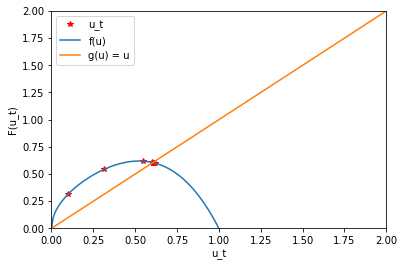
\includegraphics[width=0.5\textwidth]{graphic_3.png}
\caption{Начальное приближение $u_0 = 0.1$, фиксированные $a=1, r=1$, $t = \overline{0,10}$ }\label{pic_2}
\end{center}
\end{figure}
	Видно, что траектория не сходится к неподвижной точке $u^* = 0$.
	\end{subsection}
	\begin{subsection}{Исследование существования циклов длинной 2 и 3}
	Дадим теоретическую сводку.
	\end{subsection}
\end{document}
